% Формат дипломной работы:
%     - шрифт 14
%     - бумага А4
%     - поля 2х2х2х2см
%     - полуторный межстрочный интервал
\documentclass[14pt]{extarticle}
\usepackage[paper=a4paper, top=2cm, bottom=2cm, right=1cm, left=3cm]{geometry}
\linespread{1.3}

% Стиль оглавления
%\usepackage{titletoc}
%\titlecontents{section}[2em]{\bfseries\addvspace{0.5em}}
%{\contentslabel[\thecontentslabel]{1.7em}}
%{}{\titlerule*[1pc]{.}\contentspage}

\usepackage[utf8]{inputenc}                % Кодировка
\usepackage[main=russian, english]{babel}  % Русский язык
\usepackage[pdftex]{graphicx}              % Картинки
\usepackage{indentfirst}                   % Отступ перед абзацами

\usepackage{amsfonts}
\usepackage{amsmath}
\usepackage{multirow}

\begin{document}
    \thispagestyle{empty}
\begin{center}
    \ \vspace{-3cm}

    
\includegraphics[width=0.5\textwidth]{title_page/msu.eps}\\

    {\small{\scshape  Московский государственный университет имени~М.~В.~Ломоносова}\\
    Факультет вычислительной математики и кибернетики}

    \vfill

    {\Large Отчет по заданию}

    \vspace{1cm}

    {\LARGE\bfseries <<Численное интегрирование многомерных функций методом~Монте--Карло>>}

    \vspace{1.5cm}

    {\scshape Вариант 2}
\end{center}

\vspace{3cm}

\begin{flushright}
    \large
    \textit{Студент 615 группы}\\
    Егоров Кирилл 
\end{flushright}

\vfill

\begin{center}
    Москва, 2022
\end{center}

\clearpage
    \tableofcontents
    \clearpage
    \section{Постановка задачи}
        Рассмотрим функцию $f(x,y,z)$, непрерывную в ограниченной замкнутой области $G\subset\mathbb{R}^3$.
        Требуется вычислить определённый интеграл:
        \begin{equation}
            I = \iiint\limits_{G} f(x,y,z)\,dx\,dy\,dz.
        \end{equation}

        В рамках варианта задания преполагаются следующие значения заданных функции $f(\cdot)$ и множества $G$:
        \begin{equation}
            \begin{aligned}
                &f(x,y,z) = \frac{1}{(1+x+y+z)^3}, \\
                &\mbox{$G$~--- область, ограниченная поверхностями: $x+y+z=1$, $x=0$, $y=0$, $z=0$.}
            \end{aligned}
        \end{equation}

    \section{Аналитическое решение}
    Посчитаем приведенный выше интеграл аналитически:
    \begin{equation}
        \begin{aligned}
        &\iiint\limits_{G}\frac{dx\,dy\,dz}{(1+x+y+z)^3}
        =\\=
        &\int\limits_{0}^{1}dx\int\limits_{0}^{1-x}dy\int\limits_{0}^{1-x-y}\frac{dz}{(1+x+y+z)^3}
        =\\=
        &\int\limits_{0}^{1}dx\int\limits_{0}^{1-x}\left.\left( -\frac{1}{2(1+x+y+z)^2} \right)\right|_{0}^{1-x-y}dy
        =\\=
        &-\frac{1}{2}\int\limits_{0}^{1}dx\int\limits_{0}^{1-x}\left(\frac{1}{4}-\frac{1}{(1+x+y)^2}\right)dy
        =\\=
        &-\frac{1}{2}\int\limits_{0}^{1}\left.\left(\frac{y}{4} + \frac{1}{1+x+y}\right)\right|_{0}^{1-x}dx
        =\\=
        &-\frac{1}{2}\int\limits_{0}^{1}\left(\frac{3}{4} - \frac{x}{4} - \frac{1}{1+x}\right)dx
        =\\=
        &-\frac{1}{2}\left.\left(\frac{3}{4}x - \frac{x^2}{8} - \mathrm{ln}(x+1)\right)\right|_{0}^{1}
        =\\=
        &\frac{\mathrm{ln}\,2}{2} - \frac{5}{16} \approx 0,\!03407359.
        \end{aligned}
    \end{equation}


    \section{Численное решение}

    Для численного решения приведенного интеграла воспользуемся методом Монте--Карло [1].

    Рассмотрим параллелепипед $\Pi=[0,1]\times[0,1]\times[0,1]$, ограничивающий область $G\subset\Pi$.
    Рассмотрим также функцию
    $$
        F(x,y,z) = \left\{\begin{aligned}
            &f(x,y,z), \mbox{при $(x,y,z)\in G,$}\\
            &0, \mbox{иначе.}
        \end{aligned}\right.
    $$
    Преобразуем искомый интеграл:
    $$
        I = \iiint\limits_{G}f(x,y,z)\,dx\,dy\,dz = \iiint\limits_{\Pi}F(x,y,z)\,dx\,dy\,dz.
    $$

    Пусть $p_1(x,y,z),\,p_2(x,y,z),\ldots$~--- случайные точки, равномерно распределённые в $\Pi$.
    Возьмём $n$ таких случайных точек.
    В качестве приближённого значения интеграла предлагается использовать выражение:
    \begin{equation}
        I \approx |\Pi|\cdot\frac{1}{n}\sum\limits_{i=1}^{n}F(p_i),
    \end{equation}
    где $|\Pi|$ --- объём параллелепипеда $\Pi$.


    \section{Программная реализация}
    В рамках задачи была реализована параллельная MPI-программа, которая принимает на вход требуемую точность и генерирует случайные точки до тех пор, пока требуемая точность не будет достигнута.
    Программа вычисляет точность как модуль разности между приближённым значением, полученным методом Монте--Карло, и точным значением, вычислинным аналитически.
    
    Программа считывает в качестве аргумента командной строки требуемую точность $\varepsilon$ и выводит четыре числа:
    \begin{enumerate}
        \item Посчитанное приближённое значение интеграла.
        \item Ошибка посчитанного значения: модуль разности между приближённым и точным значениями интеграла.
        \item Количество сгенерированных случайных точек.
        \item Время работы программы в секундах.
    \end{enumerate}

    Время работы программы измеряется следующим образом. Каждый MPI-процесс измеряет своё время выполнения, затем среди полученных значений берётся максимум.

    В рамках варианта параллельные процессы генерируют случайные точки независимо друг от друга.
    Все процессы вычисляют свою часть суммы по формуле, затем вычисляется общая сумма с помощью операции редукции.

    После чего вычисляется ошибка (разность между посчитанным значением и точным значением, вычисленным аналитически).
    В случае если ошибка выше требуемой точности, которую подали на вход программе, то генерируются дополнительные точки и расчёт продолжается.

    Для обеспечения генерации разных последовательностей точек в разных MPI-процессах генератор псевдослучайных чисел инициализируется разными числами.

    Листинг кода программы представлен в приложении.

    \section{Запуск программы на системе Polus}
    Данная программа была запущена на системе Polus для различного числа MPI-процессов и различных значений входного параметра $\varepsilon$.
    Результаты работы, усреднённые по 100 запускам каждый, приведены в таблице ниже.

    \begin{table}[h]
        \small
        \begin{tabular}{|l|l|l|l|l|}
        \hline
        Точность $\varepsilon$ & Число MPI-процессов & Время работы программы (с) & Ускорение & Ошибка \\
        \hline
        \hline
        \multirow{3}{*}{$3,\!0\cdot 10^{-5}$} & 1 & 0.02 & 1 & $1,\!39\cdot 10^{-5}$ \\ \cline{2-5} 
                               & 4 & 0.12 & 0.16 & $1,\!77\cdot 10^{-5}$ \\ \cline{2-5} 
                               & 16 & 0.02 & 1 & $1,\!76\cdot 10^{-5}$ \\ \cline{2-5}
                               & 32 & 0.25 & 0.08 & $1,\!52\cdot 10^{-5}$ \\ \hline
        \multirow{3}{*}{$5,\!0\cdot 10^{-6}$} & 1 & 0.04 & 1 & $3,\!09\cdot 10^{-6}$ \\ \cline{2-5}
        & 4 & 1.04 & 0.04 & $3,\!09\cdot 10^{-6}$ \\ \cline{2-5} 
        & 16 & 0.18 & 0.22 & $2,\!75\cdot 10^{-6}$ \\ \cline{2-5}
        & 32 & 0.26 & 0.15 & $1,\!65\cdot 10^{-6}$ \\ \hline
        
        \multirow{3}{*}{$1,\!5\cdot 10^{-6}$} & 1 & 0.08 & 1 & $7,\!7\cdot 10^{-7}$ \\ \cline{2-5}
        & 4 & 0.02 & 4 & $7,\!1\cdot 10^{-7}$ \\ \cline{2-5} 
        & 16 & 0.08 & 1 & $8,\!5\cdot 10^{-7}$ \\ \cline{2-5}
        & 32 & 0.26 & 0.3 & $7,\!4\cdot 10^{-7}$ \\ \hline
        \end{tabular}
    \end{table}

    Исходя из результатов, видим что в силу быстроты (по операциям) генерации псевдослучайных чисел и подсчета функции, блокирующие операции синхронизации MPI-процессов замедляют работу исходного алгоритма.
    Анализируя таблицу, можно найти всего один результат, где время работы параллельного алгоритма ниже, чем у однопоточного.
    При этом, даже в нем видно, что при увеличении числа процессов, эффективность алгоритма снижается.

    Ниже представлены данные об ускорении в графическом виде.

    \begin{center}
        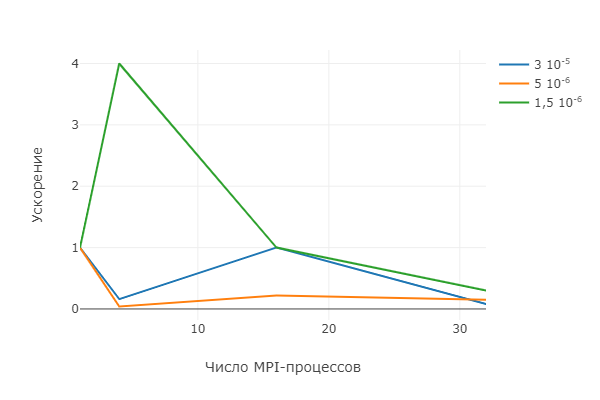
\includegraphics[width=0.8\linewidth]{newplot.png}
        \newline
        Рис. 1: Зависимость ускорения от числа процессоров для каждого значения~$\varepsilon$.
    \end{center}
\clearpage
    \begin{thebibliography}{9}
            \bibitem{math}Бахвалов Н.С., Жидков Н.П., Кобельков Г.М. ЧИСЛЕННЫЕ МЕТОДЫ. --- M.:Наука, 1987.
            \bibitem{a} Параллельные вычисления (Воеводин В.В., Воеводин Вл.В.) --- Спб, изд-во <<БХВ-Петербург>>, 2002
            \bibitem{b} IBM Polus. --- http://hpc.cs.msu.su/polus
    \end{thebibliography}
\clearpage
    \begin{verbatim}
#include <mpi.h>
#include <stdio.h>
#include <stdlib.h>
#include <time.h>
#include <math.h>
        
const int ROOT = 0;
        
const double INTEGRAL = log(2) / 2.0 - 0.3125;
        
// drand returns a double number in boundaries [0, 1.0]
double
drand() {
    return (double)rand()/(double)RAND_MAX;
}
        
// integrand returns the integrand function
double
integrand() {
    double x = drand();
    double y = drand();
    double z = drand();
    if ((y < 0) || (z < 0) || (x + y + z > 1)) {
        return 0;
    }
    double denominator = 1.0 + x + y + z;
    return 1.0 / (denominator * denominator * denominator);
}
        
double
update_integral(double prev, int prev_count,
    double add, int add_count) {
    return prev * ((double)prev_count/prev_count+add_count) +
        add / (prev_count+add_count));
}
        
int
main(int argc, const char** argv)
{
    int rank, size;
    MPI_Init(NULL, NULL);
    MPI_Comm_rank(MPI_COMM_WORLD, &rank);
    MPI_Comm_size(MPI_COMM_WORLD, &size);
        
    if (argc != 2) {
        if (rank == ROOT) {
            fprintf(stderr, "Precision is not provided\n");
        }
        MPI_Finalize();
        return 0;
    }
            
    double precision;
    if (rank == ROOT) {
        sscanf(argv[1], "%lf", &precision);
    }
        
    int start_time = time(NULL);
    srand(start_time + 100*rank);
        
    double integral = 0.0;
    double error;
    int total_parts = 0;
        
    int next = 1;
    while (next) {
        double part = integrand();
        double part_sum;
        MPI_Reduce(&part, &part_sum, 1, MPI_DOUBLE, 
            MPI_SUM, ROOT, MPI_COMM_WORLD);
        if (rank == ROOT) {
            integral = update_integral(integral, total_parts,
                part_sum, size);
            total_parts = total_parts + size;
            if (integral > INTEGRAL) {
                error = integral-INTEGRAL;
            } else {
                error = INTEGRAL-integral;
            }
            if (error < precision) {
                next = 0;
            }
        }
        MPI_Bcast(&next, 1, MPI_INT, ROOT, MPI_COMM_WORLD);
    }
        
    if (rank == ROOT) {
        printf("Integral=%.10f\n", integral);
        printf("Error=%.10f\n", error);
        printf("PointsCount=%d\n", total_parts);
        int finish_time = time(NULL);
        printf("Time=%d s\n", finish_time-start_time);
    }
        
    MPI_Finalize();
}
    \end{verbatim}

\end{document}